
\begin{frame}{Multivariate Verteilungen}
Literatur:  Fahrmeir, Hammerle und Tutz: Multivariate statistische Verfahren. De Gruyter, 1996., Kap 2,  Anhang A11 
\vspace{1cm}

Wir betrachten Zufalls--Vektoren $\X$   mit der mehrdimensionale Dichte-- und Verteilungsfunktion:  
\begin{eqnarray*}
f: \R^n &\rightarrow & \R   \\
F:  \R^n &\rightarrow & \R   
\end{eqnarray*}
Die Kovarianzmatrix von $\X$ wird mit $ V(\X) = \Sigma$ bezeichnet  

\end{frame}

\begin{frame}{Spektralzerlegung der Kovarianzmatrix $\Sigma$}
\[
\Sigma = P L P^T\text{\ \ und\ \ }\Sigma^{-1} = P L^{-1}P^T,
\]
$P$: die orthogonale Matrix der orthonormalen Eigenvektoren ist,

L: Diag($\lambda_1,\ldots,\lambda_p)$ die Diagonalmatrix der
Eigenwerte.
\[
c^2 = (\X - \mu)^T P L^{-1/2} L^{-1/2}P^T(\X-\mu) = \Y^T L^{-1}\Y =
\sum^p_{i=1}\frac{y^2_i}{\lambda_i},
\]
$\Y = P^T(\X-\mu)$.\\

Die Gleichung $\sum^p_{i=1}\frac{y_i^2}{\lambda_i} = c^2$ ist eine
Ellipsoidengleichung mit den Hauptachsenl\"{a}ngen
$\sqrt{\lambda_i}c$
\[
\Y = (v^T_1(\X - \mu),\ldots,v_p^T(\X-\mu)),
\]
sind Projektionen von $\X-\mu$ auf die Eigenvektoren
$v_1,\ldots,v_p$.
\end{frame}


\begin{frame}\frametitle{Sph\"{a}rische und  Elliptische Verteilungen}
 Verallgemeinerung von eindimensionalen Dichten durch
Rotation um Zentrum $x_0$: \\ f sei symmetrisch um 0

\[
f(\x)=const \cdot g(\sqrt{\x^T \x})
\]

Verallgemeinerung auf elliptische Verteilungen:

\[
f(\x)=|\Sigma|^{-\frac{1}{2}}\,\,(g(\x-\mu)'\Sigma^{-1}\,\,g(\x-\mu)) \cdot const
\]

Kurven gleicher Dichte sind Ellipsen.
%%----------------
\end{frame}

%\newpage
\begin{frame}\frametitle{Dichte der multivariaten Normalverteilung}
\[
f(\x)=\frac{1}{(2\pi)^{p/2}\mid\Sigma\mid^{1/2}}
\exp\left\{-\frac{1}{2}(\x-\mu)^T\Sigma^{-1}(\x-\mu)\right\},
\]

$\mu^T = (\mu_1,\ldots,\mu_p)  = E(\X^T)$ Erwartungswert.

$\Sigma$: Kovarianzmatrix \vspace{0.5cm}

H\"{o}henlinien der Normalverteilung:
\[
(\x - \mu)^T\Sigma^{-1}(\x-\mu) = c^2,
\]
\end{frame}

\begin{frame}{Normalverteilungsdichte I}
%\begin{minipage}{25cm}
\begin{center}
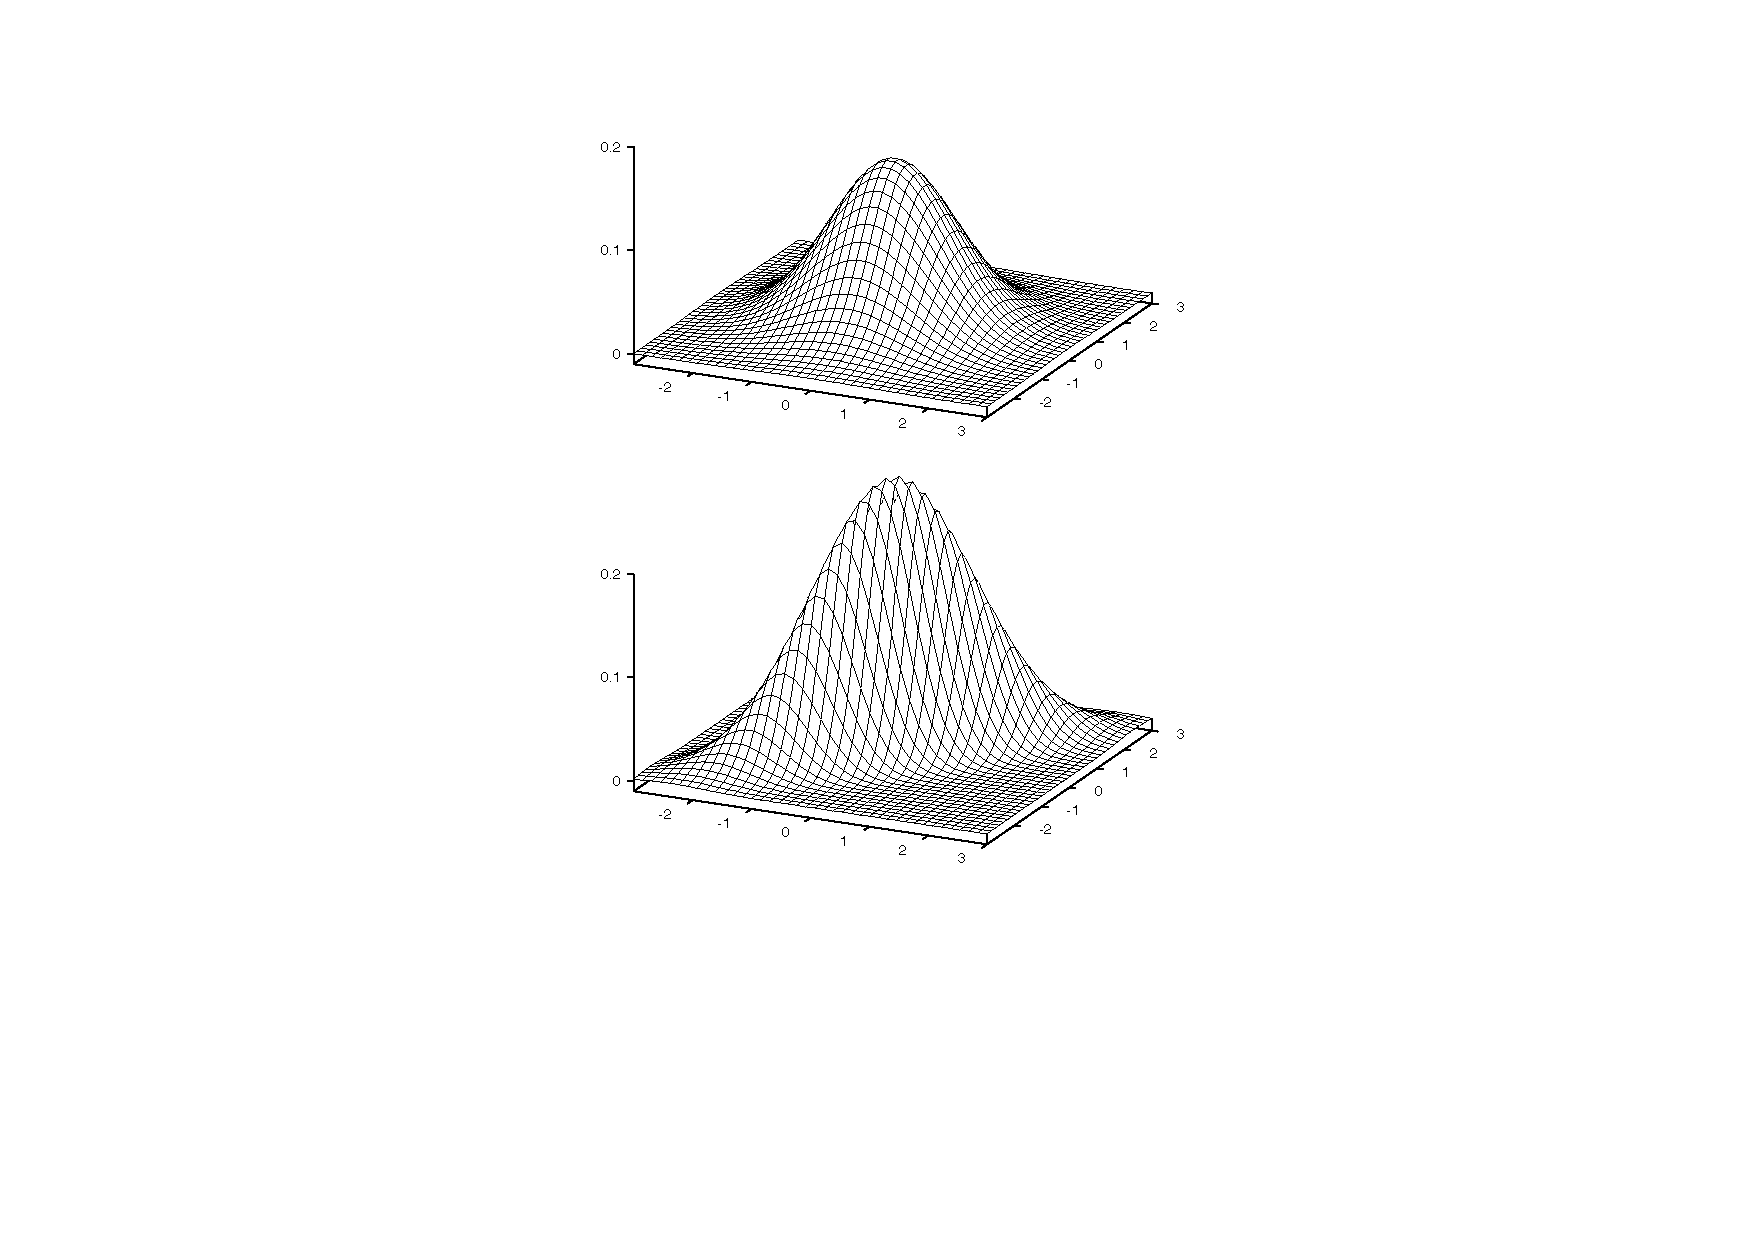
\includegraphics[scale=0.5]{eps1.pdf}
\end{center}
%\end{minipage}
\end{frame}

\begin{frame}{Normalverteilungsdichte II }
%\begin{minipage}{25cm}
\begin{center}
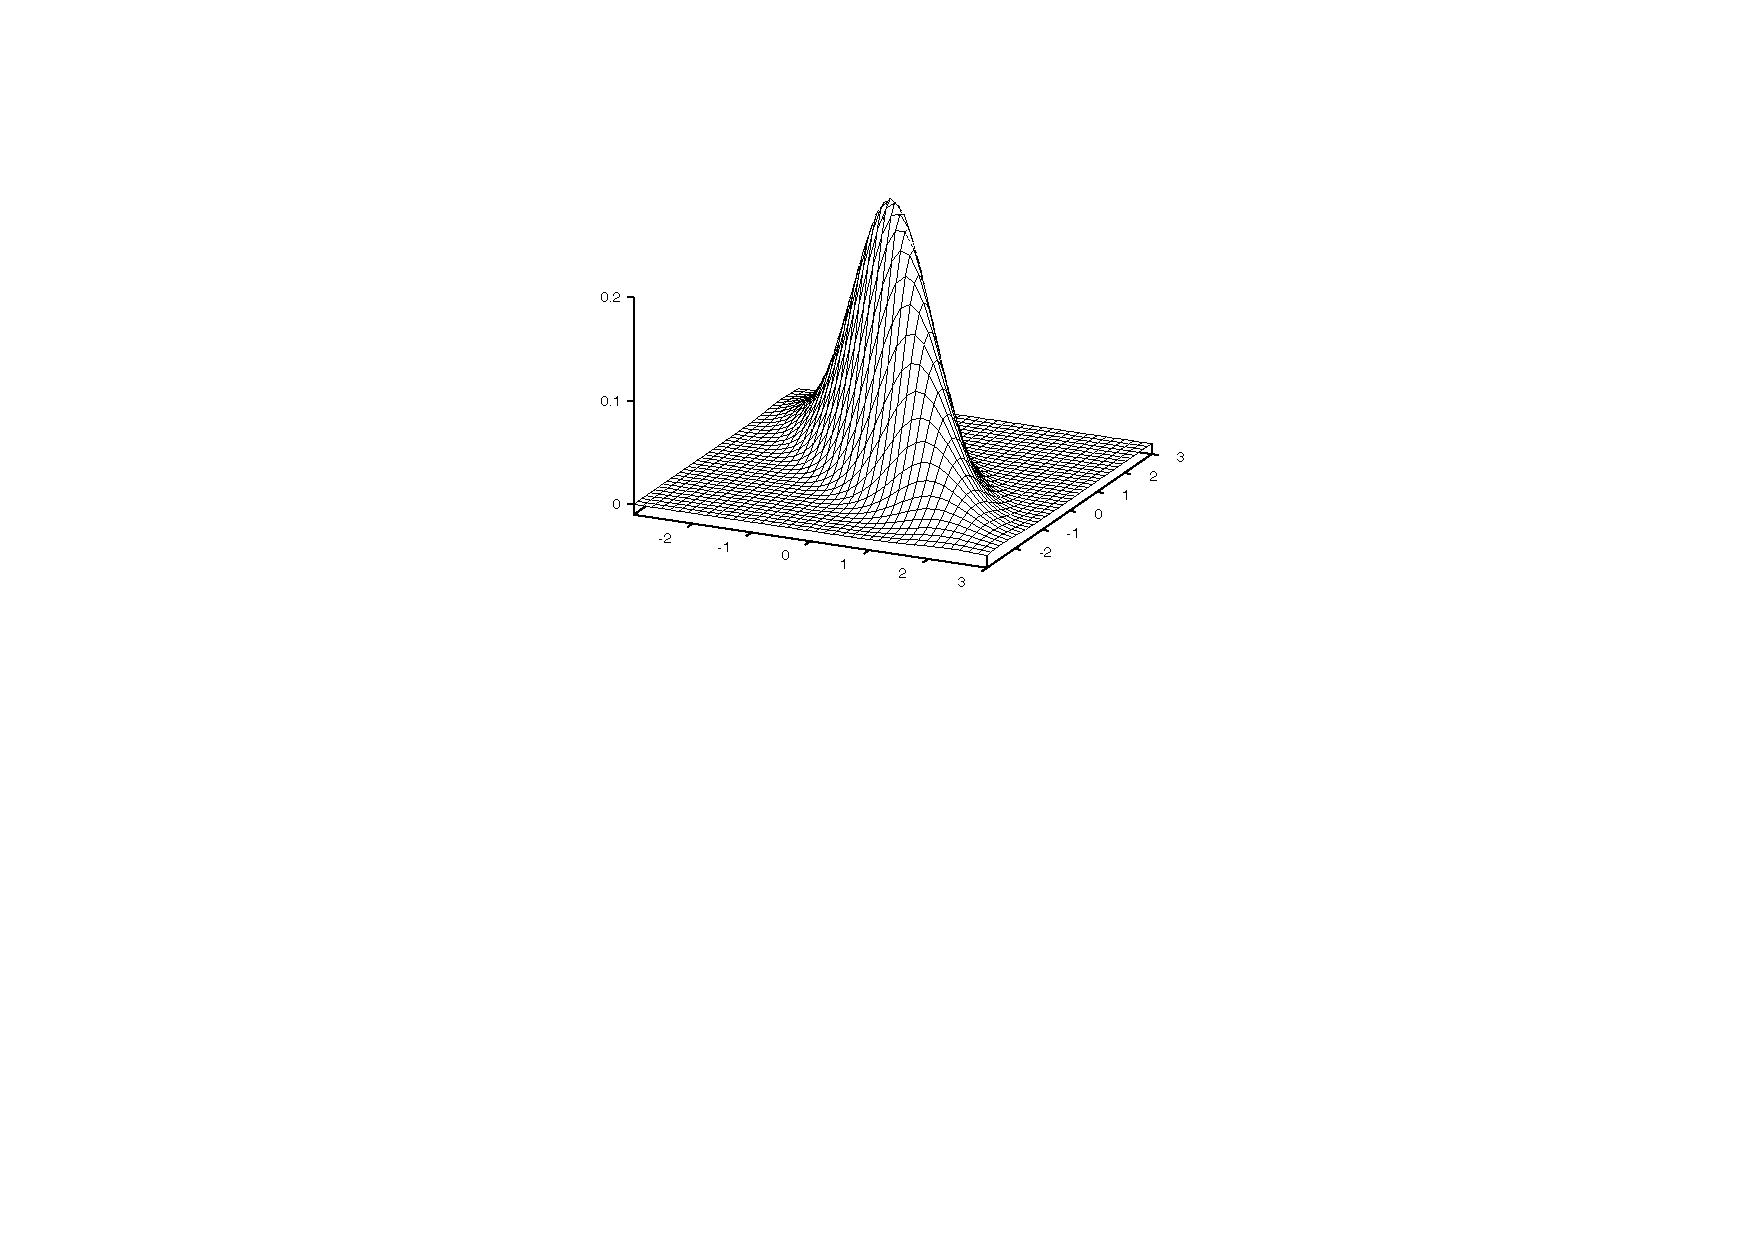
\includegraphics[scale=0.5]{pics/eps2.pdf}
\end{center}
%\end{minipage}
\end{frame}



\begin{frame}\frametitle{Einige Eigenschaften}
\begin{itemize}
\item Gilt $\X\sim N_p(\mu,\Sigma)$, dann ist $\Y = A \X + b$ mit
$(q\times p)$--Matrix $A$ und \newline $(q\times 1)$--Vektor ${\bf
b}$ wiederum nor\-mal\-ver\-teilt mit $\Y\sim N_q(A\mu + b, A\Sigma
A^T)$.
\item Gilt $\X\sim N_p(\mu,\Sigma)$, dann ist $\Y = \Sigma^{-1/2}(x-\mu)$
stan\-dard\-nor\-mal\-ver\-teilt, d.h. $\Y\sim N_p({\bf 0},I)$. Die
quadratische Form $(\X-\mu)^T\Sigma^{-1}(\X-\mu)$ ist damit
$\chi^2$--verteilt, $(\X-\mu)^T\Sigma^{-1}(\X-\mu)\sim\chi^2(p)\ .$
\end{itemize}
\end{frame}

\begin{frame}\frametitle{Einige Eigenschaften}
\begin{itemize}
\item Sei $\X\sim N(\mu,\Sigma)$ partitioniert in $\X^T =
(\X^T_1,\X^T_2)$ mit zugeh\"{o}rigen Partitionen
%\[
\begin{eqnarray*}%{ccc}
  \mu^T & = & (\mu^T_1, \mu^T_2),\\
  \Sigma & = &
\left(
  \begin{array}{cc}
    \Sigma_{11} & \Sigma_{12}\\
    \Sigma_{21} & \Sigma_{22}
  \end{array}
\right).
\end{eqnarray*}
%\]
Dann gilt f\"{u}r die bedingte Verteilung
\[
\X_2\mid \X_1\sim N(\mu_{2.1},\Sigma_{2.1}),
\]
wobei
%\[
\begin{eqnarray*}%{rcl}
\mu_{2.1} & = & \mu_2 + \Sigma_{21}\Sigma_{11}^{-1} (x_1 - \mu_1),\\
\Sigma_{2.1} & = & \Sigma_{22} -
\Sigma_{21}\Sigma_{11}^{-1}\Sigma_{12}.
\end{eqnarray*}
%\]
\end{itemize}
\end{frame}
%%----------------

%\newpage
\begin{frame}\frametitle{Wishart--Verteilung}
Seien $x_1,\ldots,x_m\sim N_p({\bf 0},\Sigma)$ und unabh\"{a}ngig.
Man betrachtet die $(p\times p)$--Matrix $M = \sum\limits^m_{i=1}x_i
x_i^T = \X^T \X$, wobei
\[
\X=\left(
\begin{array}{c}
x^T_1\\
\vdots\\
x^T_m.
\end{array}
\right)
\]
Die $(p\times p)$--Matrix $M = \sum\limits^m_{i=1}x_ix_i^T$ besitzt
eine Wishart--Verteilung mit den Parametern $\Sigma$ und $m$, $M\sim
W_p(\Sigma,m)$.
\\Die Standardform der Verteilung liegt
vor, wenn $\Sigma = I$ gilt. Gilt $M =
\sum\limits^m_{i=1}x_ix_i^T\sim W(\Sigma,m)$, erh\"{a}lt man f\"{u}r
$\Sigma^{-1/2}M\Sigma^{-1/2} = \sum\limits^m_{i=1}(\Sigma^{-1/2}x_i)
(\Sigma^{-1/2}x_i)^T \sim W_p(I,m)$.
\end{frame}



\begin{frame}{SSP--Matrix}
$X$ besitzt die Form einer Datenmatrix mit $m$ unabh\"{a}ngigen
Wiederholungen einer $p$--dimensionalen nor\-mal\-ver\-teil\-ten
Gr\"{o}{\ss}e. $M$ ist daher die SSP--Matrix (Matrix of sums of
squares and products). Sei $x^T_i = (x_{i1},\ldots,x_{im})$, dann
gilt

\[
\X=\left(
\begin{array}{c}
x_1^T\\
\vdots\\x^T_m
\end{array}
\right)=[x_{(1)},\ldots,x_{(m)}],
\]

wobei $x_{(j)}^T = (x_{1j},\ldots,x_{mj})$ zur Komponente $j$
geh\"{o}rt.
\end{frame}

\begin{frame}\frametitle{SSP--Matrix II}
\scriptsize
Man erh\"{a}lt
  \begin{eqnarray*}%{rcl}
M  =  (m_{ij}) & = & \X^T \X = \left(
    \begin{array}{c}
    x^T_{(1)}\\ \vdots \\ x_{(p)}^T
    \end{array} \right)
%
[x_{(1)},\ldots,x_{(p)}]\\[0.5cm] & = &
\left(
    \begin{array}{cccc}
    x^T_{(1)}x_{(1)} & x^T_{(1)}x_{(2)}& \ldots & x^T_{(1)}x_{(p)}\\
    x_{(2)}^Tx_{(1)}\\
    \vdots \\
    x^T_{(p)}x_{(1)} & & &x^T_{(p)}x_{(p)}
    \end{array}
\right)
  \end{eqnarray*}
mit
\begin{eqnarray*}%{rcl}
x^T_{(j)}x_{(j)} & = & \sum^m_{i=1}x^2_{ij}.\\
x^T_{(j)}x_{(s)} & = & \sum^m_{i=1}x_{ij}x_{is}.
\end{eqnarray*}
\end{frame}

\begin{frame}\frametitle{Eigenschaften}
%\footnotesize
\scriptsize
\begin{enumerate}
\item [1.] Sei \[M\sim W(\Sigma,m) \;\Longrightarrow \;E(M)= m\Sigma\]
\item [2.] F\"{u}r $p = 1$ gilt $M = \sum\limits^m_{i=1}x^2_i$,
wobei $x_i\sim N(0,\sigma^2)$, so dass $M/\sigma^2 =
\sum\limits^m_{i=1}(x_i/\sigma)^2$ eine $\chi^2(m)$--Verteilung
besitzt. Die Wishart--Verteilung $W_1(\sigma^2, m)$ ist somit
\"{a}quivalent zur $\sigma^2\chi^2(m)$--Verteilung.
\item [3.] Gelte $M = \X^T \X \sim W_p(\Sigma,m)$ und $B$ sei
$(p\times q)$--Matrix, dann gilt mit $\Y = \X B$
\[
B^T M B = B^T \X^T \X B = \Y^T \Y \sim W_q(B^T\Sigma B,m).
\]

\item [4.] Als Spezialfall von (3) ergibt sich die Verteilung von
quadratischen Formen. Gilt $M\sim W_p(\Sigma, m)$ und $a$ ist fester
Vektor mit $a^T\Sigma a \neq 0$, dann gilt
\[
\frac{a^T M a}{a^T\Sigma a} \sim \chi^2(m) = W_1(a^T\Sigma a,m).
\]

\item [5.] Gilt $M_1 \sim W_p(\Sigma, m_1),\ M_2 \sim W_p(\Sigma, m_2)$
und $M_1$ und $M_2$ sind unabh\"{a}ngig, dann gilt
\[
M_1 + M_2 \sim W_p(\Sigma, m_1 + m_2).
\]
\end{enumerate}
\end{frame}


\begin{frame}\frametitle{Hotellings $T^2$--Verteilung}
{\bf Bestimmung:}

Sei $d \sim N_p(0,I)$ und $M \sim W_p(I,m)$ und $d$ und $M$ seien
unabh\"{a}ngig, dann folgt
\[
m d^T M^{-1}d \sim T^2(p,m)
\]
Hotellings $T^2$--Verteilung, wobei $p$ die Dimension des Vektors
unabh\"{a}ngiger Normalverteilungen ist und $m$ die Anzahl der
Komponenten der Wishart--Verteilung.

Allgemeiner seien $x$ und $M$ unabh\"{a}ngig mit $x \sim
N_p(\mu,\Sigma)\ ,\ M \sim W_p(\Sigma, m)$, dann erh\"{a}lt man
\[
m(x-\mu)^TM^{-1}(x - \mu) \sim T^2(p,m)\ .
\]
\end{frame}


\begin{frame}\frametitle{Weitere Eigenschaften und Anwendungen}
\footnotesize
\begin{enumerate}
\item [1.] $T^2$ und t-Verteilung\\
Die $T^2(1,m)$--Verteilung entspricht dem Quadrat der
$t(m)$--Verteilung und damit der $F(1,m)$--Verteilung.

\item [2.] $T^2$ und $F$--Verteilung\\
Genereller gilt eine \"{A}quivalenz zwischen der $T^2$--Verteilung
und der $F$--Verteilung in der Form
\[
T^2(p,m)\ {\hat=}\{(mp)/(m-p+1)\} F(p, m-p + 1)\ .
\]

bzw.

\[F(p,s)=\frac{s}{s+p-1}\,\,T^2(p,s+p-1)\]

\item [3.] Verteilung der empirischen Mahalanobis--Distanz zwischen $\bar{x}$
und $\mu$. Aus (2) folgt wegen
\begin{eqnarray*}%{ccc}
  (n-1) (\bar{x} - \mu)^T S^{-1} (\bar{x}-\mu) & \sim & T^2(p,n-1) \\
  \frac{n-p}{p}(\bar{x}-\mu)^T S^{-1} (\bar{x} - \mu) & \sim & F(p, n-p)\ .
\end{eqnarray*}

\end{enumerate}
\end{frame}
%%----------------

%\newpage

\begin{frame}\frametitle{Wilks $\Lambda$}
Wilks $\Lambda$--Verteilung erh\"{a}lt man aus zwei unabh\"{a}ngigen
Wishart--verteilten Gr\"{o}{\ss}en $A\sim W_p(I, m),\;B\sim W_p(I,
n),\;m\ge p$. Die Gr\"{o}{\ss}e
\[
\Lambda=\frac{\mid A\mid}{\mid A + B\mid} \sim \Lambda(p, m, n)
\]
folgt der Wilks--Verteilung $\Lambda(p, m, n)$ mit Parametern $p, m,
n$.

Durch Erweitern mit  $\mid A\mid^{-1}$ folgt wegen $\mid A B\mid=
\mid A\mid\ \mid B\mid$ f\"{u}r $\Lambda$ die Darstellung
$\Lambda=\mid I + A^{-1}B\mid^{-1}$.\\
\end{frame}

\begin{frame}\frametitle{Eigenschaften}
\begin{enumerate}
\item [1.] F\"{u}r den eindimensionalen Spezialfall $A\sim
\chi^2(1),\;B\sim\chi^2$(1) ergibt sich die Beta--Verteilung
$\Lambda(1, 1, 1)\,{\hat =}\,B(0.5, 0.5)$.
\item [2.] F\"{u}r $p=1$ besitzt $A$ eine $\chi^2(m)$--Verteilung und
$B$ eine $\chi^2(n)$--Verteilung, so dass
\[
\Lambda(1, m, n)=B(m/2, n/2).
\]
\item [3.] Die Verteilungen $\Lambda(p, m, n)$ und $\Lambda(n, m+n-p, p)$ sind identisch.
\item [4.] Die Verteilung von $\Lambda(p, m, n)$ ist identisch mit der Verteilung des Produkts
\[
u_1\cdot\ldots\cdot u_n,
\]
wobei $u_i\sim B((m+i-p)/2, p/2), i=1, \ldots, n$.
\item [5.] Die Verteilung von $\Lambda(p,m,1)$ ist \"{a}quivalent zu $B((m+1-p)/2, p/2)$.
\end{enumerate}
\end{frame}


\begin{frame}\frametitle{Diskrete Multivariate
Verteilungen}

\begin{itemize}
\item {\bf Multinomialverteilung}
\item {\bf Multivariate Hypergeometrische Verteilung} \\
Diese Verteilung entspricht der Verallgemeinerung des "Ziehen ohne
Zur\"{u}cklegen". Gezogen werden n  aus N Objekten, die in K Klassen
zerfallen. Es sind jeweils $N_1,\ldots,N_K$ Objekte vorhanden. Die
Wahrscheinlichkeitsfunktion ist
$$ P(X_1=n_1,\ldots,X_K=n_K) = \frac {\prod_{k=1}^K {N_k \choose
n_k}}{{N\choose n}} \;\;\mbox{f\"{u}r} \sum n_k = n
$$
\end{itemize}
\end{frame}

